\section{Entwicklung der Mitarbeiteransicht}

\subsection{Einleitung}

Der Umfang dieses Projekts besteht in der Entwicklung einer Mitarbeiteransicht, die eine benutzerfreundliche und effiziente Verwaltung von Buchungsdaten ermöglicht. Dies umfasst die Gestaltung einer klaren und intuitiven Benutzeroberfläche, die den Anforderungen der Equilibria GmbH entspricht, sowie die Integration moderner Technologien zur Datenverarbeitung und -darstellung. Ein besonderer Fokus liegt dabei auf der Implementierung grafischer Abfragemöglichkeiten für eine einfache und effiziente Verwaltung der Daten. Aus dieser Zielsetzung ergibt sich folgende zentrale Forschungsfrage:
\newline

\begin{center}
	
	\textbf{{Wie kann eine Mitarbeiteransicht entwickelt und gestaltet werden, die durch eine intuitive Benutzeroberfläche sowie effiziente und sichere Schnittstellen die Verwaltung von Buchungsdaten optimiert?}}
    
\end{center}

Zur Beantwortung wird eine systematische Untersuchung bestehender Frontend-Technologien durchgeführt.

\subsection{Grundlagen der Webentwicklung}

\subsubsection{Geschichte der Webentwicklung}
DDas World Wide Web wurde 1989 von Tim Berners-Lee am CERN entwickelt, um Wissenschaftlern eine Plattform zum weltweiten Austausch von Informationen unabhängig vom Speicherort zu bieten. Es sollte eine einheitliche und leicht zugängliche Möglichkeit für die Verbreitung von Wissen schaffen.\textit{\cite{cern_birth_web}}

\subsubsection{Web 1.0 (1993–2003)}

Web 1.0 war die erste Phase des Internets und diente ausschließlich der Anzeige von Informationen. Es basierte auf Technologien wie HTML, HTTP und CSS, die eine einfache Struktur und Darstellung von Websites ermöglichten. Die Interaktion mit den Inhalten war nicht möglich, was Web 1.0 zu einem passiven Medium machte. Die Ladezeiten waren lang, und die Inhalte wurden unidirektional übertragen.\textit{\cite{jacksi2019development}}

\subsubsection{Web 2.0 (2004–2014)}

Der Begriff Web 2.0 wurde 2004 von Dale Dougherty geprägt und markierte den Übergang zu interaktiven und nutzergenerierten Inhalten. Durch die Einführung von Technologien wie JavaScript, XML und Ajax konnten Nutzer nicht nur Inhalte lesen, sondern auch aktiv erstellen und teilen. Diese Phase legte den Grundstein für soziale Netzwerke und Plattformen wie Facebook oder YouTube. Allerdings brachte sie auch neue Herausforderungen wie Datenschutzrisiken und Sicherheitslücken mit sich.\textit{\cite{jacksi2019development}}

\subsubsection{Web 3.0 (2014-Heute)}

Web 3.0, auch bekannt als das Semantische Web, zeichnet sich durch intelligente Inhalte und KI-Integration aus. Technologien wie RDF und SPARQL ermöglichen es Computern, Daten zu analysieren und personalisierte, kontextbezogene Ergebnisse zu liefern. Anwendungen wie virtuelle Assistenten oder KI-gestützte Tools nutzen diese Technologien. Darüber hinaus erweitert Web 3.0 das Nutzererlebnis durch 3D-Grafiken und dynamische Anwendungen, was neue Möglichkeiten für Interaktionen im Internet schafft.\textit{\cite{jacksi2019development}}

\subsection{Unterschied zwischen Frontend und Backend}

Frontend und Backend arbeiten eng zusammen, um eine vollständige Website zu bilden. Das Frontend vereinfacht und visualisiert die komplexen Prozesse des Backends für den Benutzer, während das Backend die notwendigen Daten und Funktionen bereitstellt, die das Frontend benötigt, um reibungslos zu funktionieren\textit{\cite{ionos_backend_frontend}}

\subsubsection{Frontend}
Das Frontend ist der sichtbare Teil einer Website, mit dem Benutzer direkt interagieren
Es umfasst:
\begin{itemize}
	\item Die grafische Benutzeroberfläche (GUI)
	\item Design-Elemente wie Layout, Farben und Typografie
	\item Interaktive Elemente wie Buttons, Formulare und Menüs
	\item Alles, was der Benutzer sieht und bedient
\end{itemize}
Frontend-Entwickler verwenden hauptsächlich HTML, CSS und JavaScript, um ansprechende und benutzerfreundliche Oberflächen zu erstellen.\textit{\cite{ionos_backend_frontend}}


\subsubsection{Backend}
Das Backend ist der \glqq unsichtbare\grqq{} Teil einer Website, der im Hintergrund arbeitet.
Es beinhaltet:
\begin{itemize}
	\item Server und Datenbanken
	\item Datenverarbeitung und -speicherung
	\item Logik und Funktionalität der Website
	\item Sicherheitsmaßnahmen und Authentifizierung
\end{itemize}
Backend-Entwickler nutzen Programmiersprachen wie PHP, Python, Java oder C\# sowie Datenbanksysteme, um die Funktionalität der Website sicherzustellen.\textit{\cite{ionos_backend_frontend}}

\subsection{Frontend-Frameworks}
\subsubsection{Was sind (Web-)Frameworks?}
Frameworks sind strukturierte Sammlungen von Bibliotheken, Werkzeugen und Klassen, die speziell für die Entwicklung von Softwareanwendungen konzipiert sind. Sie vereinfachen die Entwicklung durch vorgefertigte Lösungen für wiederkehrende Aufgaben wie Datenverarbeitung, Authentifizierung, Benutzeroberflächengestaltung oder API-Integration.\textit{\cite{madurapperuma2022state, shetty2020review}}

\textbf{Aufbau und Funktion:}
\begin{itemize}
	\item Frameworks basieren oft auf einer Architektur wie MVC (Model-View-Controller) oder MVVM (Model-View-ViewModel), die den Code in Module aufteilt, um die Wartbarkeit und Wiederverwendbarkeit zu erhöhen. Dies reduziert die Komplexität und verbessert die Skalierbarkeit.\textit{\cite{madurapperuma2022state, rathinam2022analysis}}
	
	\begin{figure}
		\centering
		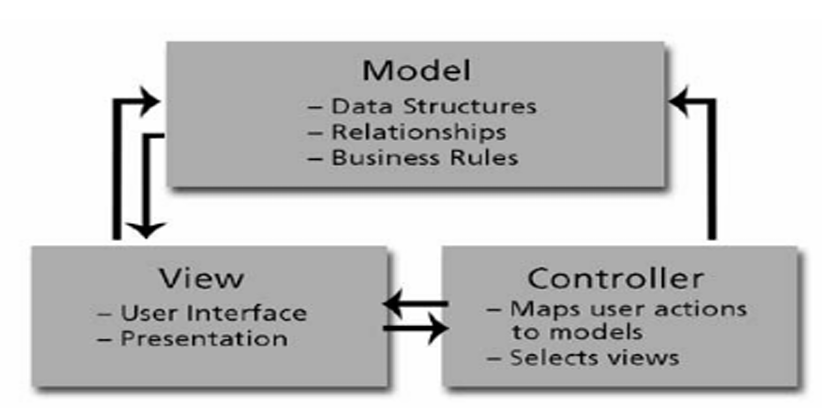
\includegraphics[width=0.5\textwidth]{images/MVC_architecture.png}
		\caption{zeigt die Model-View-Controller (MVC)-Architektur, die eine klare Trennung zwischen Daten, Benutzeroberfläche und Logik bietet. \textit{\cite{madurapperuma2022state}}}
	\end{figure}
	
	\item Sie bieten standardisierte Funktionen wie Datenbindung (z. B. in Angular oder Vue.js), virtuelle DOM-Verarbeitung (z. B. in React) und Werkzeuge für die Performance-Optimierung.\textit{\cite{awasthiresearch}}
\end{itemize}

\subsubsection{Vorteile von Webframeworks}
\begin{itemize}
	\item \textbf{Beschleunigte Entwicklung}: Frameworks wie Angular, React oder Vue.js bieten Module und Werkzeuge, die Entwicklern ermöglichen, weniger Code zu schreiben und gleichzeitig hohe Qualität zu gewährleisten.\textit{\cite{hutagikar2020analysis}}
	
	
	\item \textbf{Flexibilität und Performance}: Technologien wie Reacts virtueller DOM oder Vue.js’ modulare Architektur ermöglichen die Erstellung dynamischer und leistungsfähiger Anwendungen.\textit{\cite{shetty2020review}}
	
	\item \textbf{Skalierbarkeit}: Backend-Frameworks wie Node.js und Frontend-Frameworks wie Angular sind speziell auf wachsende Anforderungen optimiert und unterstützen einfache Erweiterungen.\textit{\cite{madurapperuma2022state}}
	
\end{itemize}

\subsubsection{Nachteile von Webframeworks}
\begin{itemize}
	\item \textbf{Lernkurve}: Frameworks wie Angular führen zusätzliche Konzepte wie TypeScript ein, die eine längere Einarbeitungszeit erfordern. Andere wie React erfordern das Verständnis von JSX und State Management.\textit{\cite{awasthiresearch, rathinam2022analysis}}
	
	
	\item \textbf{Abhängigkeit von der Auswahl}: Die Wahl eines falschen Frameworks kann zu Schwierigkeiten in der Entwicklung und Performance-Problemen führen. Zum Beispiel ist Angular ideal für große Anwendungen, während Vue.js besser für kleinere Projekte geeignet ist.\textit{\cite{rathinam2022analysis}}
	
\end{itemize}

\begin{figure}
	\centering
	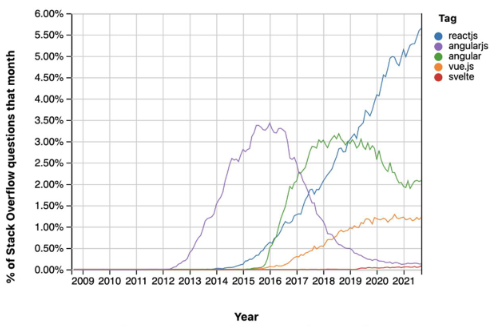
\includegraphics[width=0.5\textwidth]{images/framework_popularity.png}
	\caption{zeigt die Popularität verschiedener Frontend-Frameworks über die Jahre, basierend auf dem Anteil der Fragen auf Stack Overflow. \textit{\cite{akivab_js_framework}}}
\end{figure}



\subsubsection{Angular}

\textbf{Einführung in Angular}
\newline
Angular ist ein quelloffenes Framework für die Frontend-Webentwicklung, das von Google entwickelt wurde. Es wurde erstmals 2010 als AngularJS eingeführt und mit Angular 2 vollständig überarbeitet. Es basiert auf TypeScript und ermöglicht die Erstellung dynamischer, skalierbarer Single-Page-Anwendungen (SPAs). Durch regelmäßige Updates bleibt Angular ein modernes Framework, das an die Anforderungen der Webentwicklung angepasst ist.\textit{\cite{madurapperuma2022state, shetty2020review, angular}} \newline


\textbf{Architektur}
\newline
Angular verwendet eine komponentenbasierte Architektur, bei der die Benutzeroberfläche in kleine, wiederverwendbare Teile (Komponenten) unterteilt wird. Jede Komponente besteht aus:

\begin{itemize}
	\item \textbf{Templates}: HTML, erweitert mit Angular-spezifischen Direktiven.
	\item \textbf{Styles}: CSS oder SCSS für das Design.
	\item \textbf{Logik}: TypeScript für die Geschäftslogik.
\end{itemize}

Komponenten werden in Modulen (\texttt{NgModules}) gruppiert, um eine bessere Organisation und Wiederverwendbarkeit zu gewährleisten. Diese Struktur fördert die Modularität und erleichtert die Wartung des Codes.\textit{\cite{hutagikar2020analysis, shetty2020review, angular}} \newline

\textbf{Hauptfunktionen von Angular}

\textbf{Datenbindung} 

Angular unterstützt sowohl Einweg- als auch Zweiweg-Datenbindung:

\begin{itemize}
	\item \textbf{Einweg-Datenbindung}: Daten fließen nur vom Model zur View.
	\item \textbf{Zweiweg-Datenbindung}: Änderungen in der View werden automatisch an das Model zurückgegeben und umgekehrt. Dies wird häufig für Formulare verwendet und reduziert den manuellen Aufwand bei der Synchronisation.\textit{\cite{hutagikar2020analysis, madurapperuma2022state, angular}}
\end{itemize}

\textbf{Vorteile von Angular}
\begin{itemize}
	\item \textbf{Skalierbarkeit}: Angular eignet sich sowohl für kleine als auch für große Projekte, dank seiner Modularität und TypeScript-Unterstützung.\textit{\cite{madurapperuma2022state, rathinam2022analysis, angular}}
	
	\item \textbf{Integrierte Tools}: Angular CLI (Command Line Interface) erleichtert die Projektinitialisierung, den Build-Prozess und das Testen. Angular Material bietet vorgefertigte UI-Komponenten, die das Design beschleunigen.\textit{\cite{hutagikar2020analysis, angular_blog}}
	
	\item \textbf{Community und Support}: Als von Google unterstütztes Framework verfügt Angular über eine aktive Entwicklergemeinschaft, regelmäßige Updates und umfassende Dokumentation.\textit{\cite{shetty2020review, angular}}
\end{itemize}

\textbf{Nachteile von Angular}
\begin{itemize}
	\item \textbf{Steile Lernkurve}: Durch die Einführung von TypeScript, Dependency Injection und einer komplexen Struktur ist Angular für Anfänger herausfordernd.\textit{\cite{madurapperuma2022state, rathinam2022analysis, angular_blog}}
	\item \textbf{Framework-Größe}: Angular ist im Vergleich zu leichtgewichtigen Frameworks wie Vue.js oft schwerer und kann dadurch die Ladezeit beeinflussen.\textit{\cite{shetty2020review, angular}}
\end{itemize}


\subsubsection{React}

\textbf{Einführung in React}
\newline
React ist eine quelloffene JavaScript-Bibliothek, die von Meta (ehemals Facebook) entwickelt wurde und hauptsächlich zur Erstellung von Benutzeroberflächen verwendet wird. Sie wurde erstmals 2013 veröffentlicht und ist besonders für die Entwicklung dynamischer Single-Page-Anwendungen (SPAs) geeignet. React basiert auf dem Konzept von Komponenten und der Verwendung eines virtuellen DOM, um die Performance zu optimieren. Es bietet eine flexible Architektur für die Entwicklung moderner Webanwendungen.\textit{\cite{rathinam2022analysis, hutagikar2020analysis, react}} \newline

\textbf{Architektur}
\newline
React verwendet eine komponentenbasierte Architektur, bei der Benutzeroberflächen in kleinere, wiederverwendbare Teile aufgeteilt werden. Diese Architektur ermöglicht eine einfache Wartung und Erweiterung von Anwendungen. Jede Komponente in React ist in JSX (JavaScript XML) geschrieben, einer Syntaxerweiterung, die HTML-ähnlichen Code innerhalb von JavaScript erlaubt.

\begin{itemize}
	\item \textbf{Virtueller DOM}: React verwendet einen virtuellen DOM, der Änderungen an der Benutzeroberfläche effizient berechnet und nur die betroffenen Teile des echten DOM aktualisiert.
	\item \textbf{JSX}: JSX ist eine Mischung aus JavaScript und HTML, die es Entwicklern ermöglicht, benutzerdefinierte UI-Komponenten zu erstellen.
	\item \textbf{Unidirektionaler Datenfluss}: Daten fließen in React in einer einzigen Richtung, was die Verwaltung und Nachverfolgbarkeit von Daten einfacher macht.\textit{\cite{rathinam2022analysis, hutagikar2020analysis, react}}
\end{itemize}

\textbf{Hauptfunktionen von React}

\textbf{Komponentenbasierte Entwicklung} 

React ermöglicht die Erstellung von wiederverwendbaren und modularen Komponenten, die sowohl die Benutzeroberfläche als auch die Logik kapseln. Dies fördert eine bessere Strukturierung und Wartbarkeit des Codes.\textit{\cite{shetty2020review, react}}

\textbf{Virtueller DOM} 

Der virtuelle DOM verbessert die Performance von React-Anwendungen, indem er Änderungen effizient berechnet und nur die betroffenen Teile des echten DOM aktualisiert. Dies reduziert die Anzahl der direkten DOM-Manipulationen erheblich.\textit{\cite{rathinam2022analysis, hutagikar2020analysis, react}}

\textbf{Vorteile von React}
\begin{itemize}
	\item \textbf{Performance}: Der virtuelle DOM und die asynchrone Verarbeitung ermöglichen eine schnelle und effiziente Benutzeroberfläche.\textit{\cite{rathinam2022analysis, react}}
	
	\item \textbf{Flexibilität und Wiederverwendbarkeit}: Die komponentenbasierte Architektur von React erleichtert die Wiederverwendung von Code und die Skalierung von Anwendungen.\textit{\cite{hutagikar2020analysis, react}}
	
	\item \textbf{Große Community und Ökosystem}: React wird von einer riesigen Entwicklergemeinschaft unterstützt, und es gibt zahlreiche Bibliotheken und Tools, die den Entwicklungsprozess verbessern.\textit{\cite{shetty2020review, react}}
\end{itemize}

\textbf{Nachteile von React}
\begin{itemize}
	\item \textbf{Zusätzliche Abhängigkeiten}: React bietet nur die grundlegende Architektur, weshalb oft zusätzliche Bibliotheken (z. B. für Routing oder State Management) benötigt werden.\textit{\cite{shetty2020review, rathinam2022analysis, react_blog}}
	
	\item \textbf{Lernkurve}: Für Entwickler, die mit JSX und der Unidirektionalität des Datenflusses nicht vertraut sind, kann React eine gewisse Lernkurve darstellen.\textit{\cite{hutagikar2020analysis, react_blog}}
\end{itemize}



\subsubsection{Vue.js}

\textbf{Einführung in Vue.js}
\newline
Vue.js ist ein progressives JavaScript-Framework, das 2014 von Evan You entwickelt wurde. Es wird häufig für die Erstellung von Benutzeroberflächen und Single-Page-Anwendungen (SPAs) verwendet. Vue.js zeichnet sich durch seine einfache Integration in bestehende Projekte und seine Flexibilität aus, wodurch es sowohl für kleine als auch große Anwendungen geeignet ist. Durch seine modulare Struktur und starke Community-Unterstützung bleibt Vue.js ein beliebtes Framework für Webentwickler.\textit{\cite{rathinam2022analysis, madurapperuma2022state, vuejs}} \newline

\textbf{Architektur}
\newline
Vue.js verwendet die Model-View-ViewModel (MVVM)-Architektur, die es ermöglicht, die Benutzeroberfläche, die Geschäftslogik und die Datenbindung effizient zu verwalten. Die Hauptbestandteile von Vue.js sind:

\begin{itemize}
	\item \textbf{Templates}: Vue.js verwendet Templates, um UI-Komponenten zu definieren. Diese Templates werden in renderbare DOM-Elemente übersetzt.
	\item \textbf{Reaktivitätssystem}: Das reaktive Datenmodell von Vue.js ermöglicht automatische Updates der Benutzeroberfläche, wenn sich die zugrunde liegenden Daten ändern.
	\item \textbf{Direktiven}: Vue.js bietet spezielle HTML-Attribute (Direktiven), die Funktionen wie Schleifen, Bedingungen und Ereignishandlungen erleichtern.\textit{\cite{hutagikar2020analysis, vuejs}}
\end{itemize}

\textbf{Hauptfunktionen von Vue.js}

\textbf{Komponentenbasierte Entwicklung} 

Wie React und Angular ermöglicht Vue.js die Erstellung von wiederverwendbaren und modularen Komponenten. Diese Struktur fördert die Organisation und erleichtert die Wartung und Erweiterung von Anwendungen.\textit{\cite{rathinam2022analysis, vuejs}}

\textbf{Reaktivitätssystem} 

Das Reaktivitätssystem von Vue.js überwacht automatisch Änderungen im Datenmodell und aktualisiert die Benutzeroberfläche entsprechend. Dies macht die manuelle DOM-Manipulation überflüssig und verbessert die Entwicklererfahrung.\textit{\cite{hutagikar2020analysis, vue_blog}}

\textbf{Vorteile von Vue.js}
\begin{itemize}
	\item \textbf{Einfache Lernkurve}: Vue.js ist einfach zu lernen, da es eine klare und intuitive Syntax bietet. Es ist besonders für Entwickler geeignet, die mit HTML, CSS und JavaScript vertraut sind.\textit{\cite{madurapperuma2022state, vuejs}}
	
	\item \textbf{Flexibilität und Modularität}: Vue.js kann sowohl für einfache Widgets als auch für komplexe Anwendungen verwendet werden. Seine modulare Struktur ermöglicht eine einfache Integration in bestehende Projekte.\textit{\cite{rathinam2022analysis, vuejs}}
	
	\item \textbf{Leichtgewichtig und performant}: Vue.js ist kleiner als Frameworks wie Angular und React, was die Ladezeit reduziert und die Performance verbessert.\textit{\cite{shetty2020review, vuejs}}
\end{itemize}

\textbf{Nachteile von Vue.js}
\begin{itemize}
	\item \textbf{Geringere Unterstützung durch große Unternehmen}: Im Gegensatz zu React und Angular wird Vue.js nicht von einer großen Organisation unterstützt, was in einigen Fällen zu Unsicherheiten führen kann.\textit{\cite{rathinam2022analysis, vue_blog}}
	
	\item \textbf{Weniger umfangreiches Ökosystem}: Während Vue.js eine starke Community hat, sind bestimmte Drittanbieter-Bibliotheken und Tools im Vergleich zu React und Angular weniger verbreitet.\textit{\cite{hutagikar2020analysis, vue_blog}}
\end{itemize}
